\section{BUSCO Results}\label{section:busco}

Results of BUSCO analysis using the sordariomycetes\_Odb12 dataset
provided by BUSCO are presented in Figure~\ref{fig:busco-counts}, and
Table~\ref{table:busco}. The results indicate that all gene sets
considered in this analysis have a BUSCO completeness of 94.1\% or
higher, with a maximum completeness of 98.4\% in the case of Braker2
and DC1. In general, Braker2 and RefSeq have the most BUSCO complete
sets of gene predictions of the three tools considered. Interestingly,
Braker2 produces far more duplicated BUSCO matches than both GeneMark
and RefSeq. Examining the BUSCO output logs, this appears to be due to
Braker2 predicting more than one coding sequence for some genes
predictions, resulting in multiple similar proteins. Interestingly,
the coding sequences in the RefSeq annotations seem to miss more genes
than the other two gene finders while also having a higher number of
fragmented BUSCO genes. This may be due to human curation of the
RefSeq datasets, or the Gnomon gene prediction pipeline used by NCBI
to produce these annotations. Further investigation is required to
determine the exact cause of this discrepancy. Finally, it appears
that \textit{T. reesei} tends to have slightly lower BUSCO
completeness than the other \textit{Trichoderma} species considered in
this analysis, regardless of gene finder used. Why this is the case is
unknown, but may be due to the evolutionary distance between
\textit{T. reesei}, the Gnomon annotation process, or potentially the
fragmented nature of the \textit{T. reesei} assembly used in this
analysis. While these results do not capture the entire set of genes
possibly present in these \textit{Trichoderma} assemblies, they do
confirm that the gene finders are at minimum predicting many
evolutionarily conserved fungal genes.

\begin{figure}
  \centering
  \begin{subfigure}{0.9\textwidth}
    \centering
    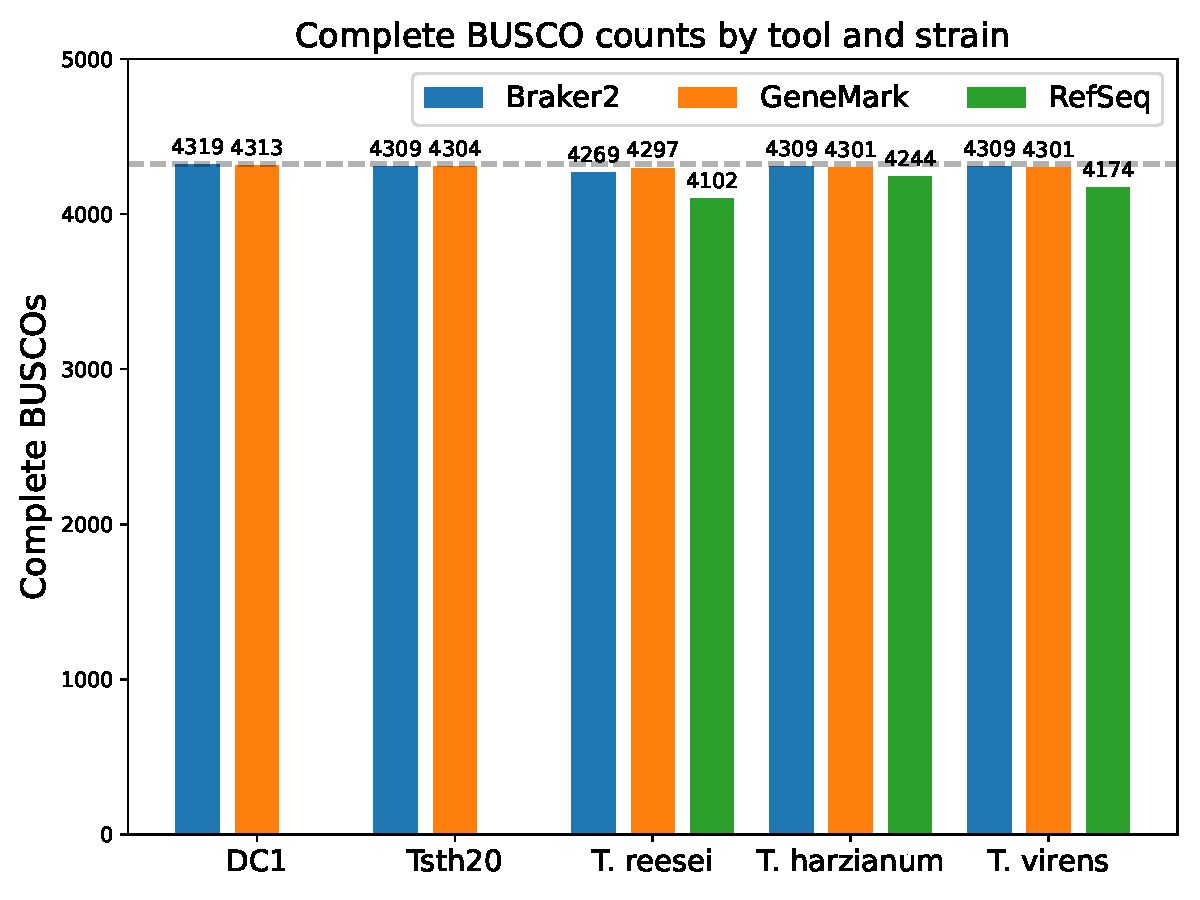
\includegraphics[width=\textwidth]{figures/busco-complete-counts.pdf}
  \end{subfigure}
  \hfill
  \begin{subfigure}{0.9\textwidth}
    \centering
    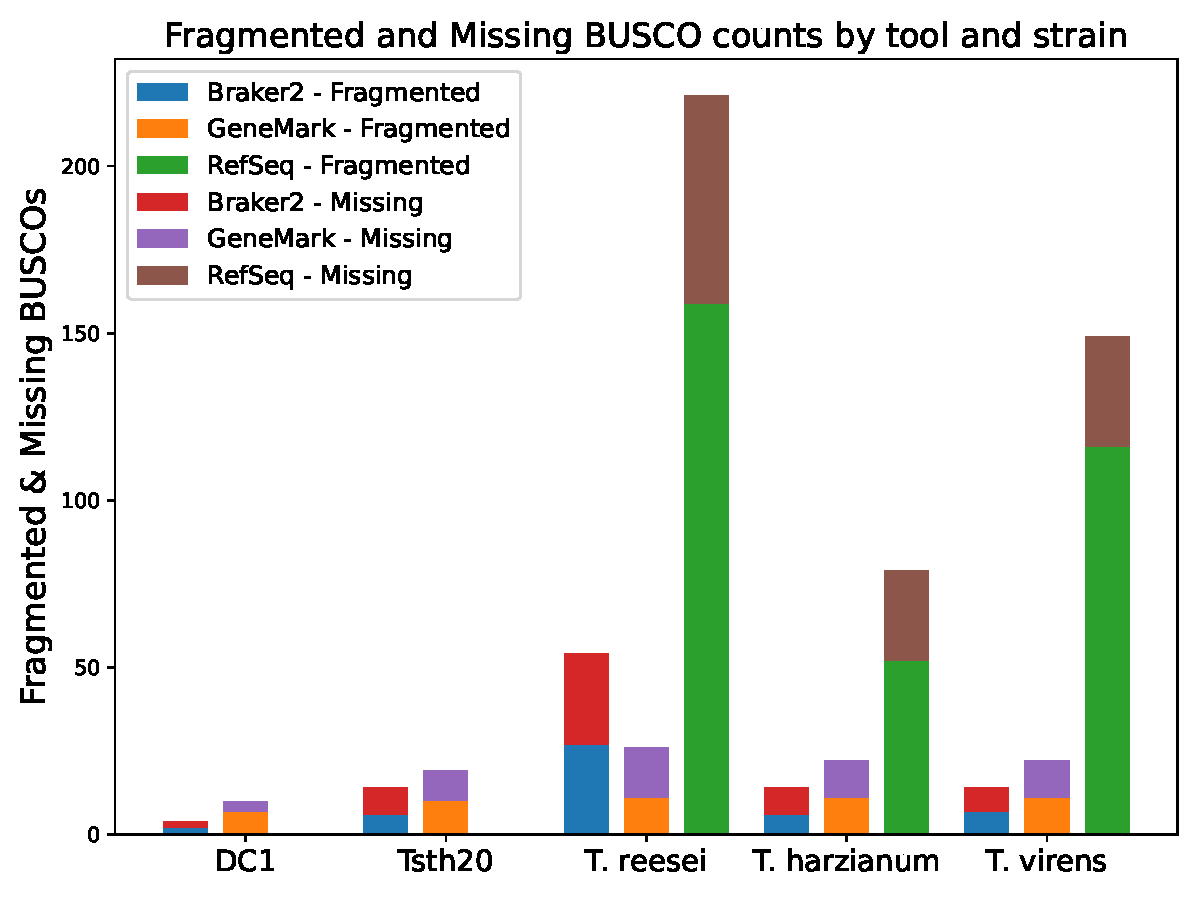
\includegraphics[width=\textwidth]{figures/busco-missing-counts.pdf}
  \end{subfigure}
  \caption[BUSCO counts]{BUSCO complete and missing gene counts for each gene finder across all \textit{Trichoderma} genome assemblies. There were a total of 4492 markers in the selected BUSCO dataset. For DC1 and Tsth20, RefSeq annotations are not available, so their values are set to 0. The selected sordariomycetes\_Odb12 dataset contains 4492 markers.}\label{fig:busco-counts}
\end{figure}

\begin{table}
  \begin{center}
    \begin{subtable}{\textwidth}
      \centering
      \begin{tabular}{|c|c|c|c|c|c|c|}
        \hline
        Strain & Complete & Single & Duplicated & Fragmented & Missing \\ \hline
        DC1 & 4419 & 3547 & 872 & 40 & 33 \\ \hline
        Tsth20 & 4416 & 3585 & 831 & 42 & 34 \\ \hline
        \textit{T. reesei} & 4321 & 3587 & 734 & 80 & 91 \\ \hline
        \textit{T. harzianum} & 4408 & 3572 & 836 & 49 & 35 \\ \hline
        \textit{T. virens} & 4409 & 3530 & 879 & 53 & 30 \\ \hline
      \end{tabular}
      \caption{Braker2}
      \vspace{0.5cm}
    \end{subtable}
    \begin{subtable}{\textwidth}
      \centering
      \begin{tabular}{|c|c|c|c|c|c|c|}
        \hline
        Strain & Complete & Single & Duplicated & Fragmented & Missing \\ \hline
        DC1 & 4415 & 4401 & 14 & 43 & 34 \\ \hline
        Tsth20 & 4409 & 4392 & 17 & 47 & 36 \\ \hline
        \textit{T. reesei} & 4351 & 4345 & 6 & 69 & 72 \\ \hline
        \textit{T. harzianum} & 4399 & 4382 & 17 & 53 & 40 \\ \hline
        \textit{T. virens} & 4391 & 4369 & 22 & 61 & 40 \\ \hline
      \end{tabular}
      \caption{GeneMark}
      \vspace{0.5cm}
    \end{subtable}
    \begin{subtable}{\textwidth}
      \centering
      \begin{tabular}{|c|c|c|c|c|c|c|}
        \hline
        Strain & Complete & Single & Duplicated & Fragmented & Missing \\ \hline
        \textit{T. reesei} & 4274 & 4267 & 7 & 112 & 106 \\ \hline
        \textit{T. harzianum} & 4383 & 4366 & 17 & 60 & 49 \\ \hline
        \textit{T. virens} & 4345 & 4321 & 24 & 92 & 55 \\ \hline  
      \end{tabular}
      \caption{RefSeq}
    \end{subtable}
  \end{center}
  \caption[BUSCO results]{Results from BUSCO using the fungal analysis option
    organized by gene finding tool. The sordariomycetes\_Odb12 dataset
    contains 4492 markers. For more information on the categories
    assigned by BUSCO, please refer to the documentation.}\label{table:busco}
\end{table}

While BUSCO matches are a good metric for general performance of gene
finders, it is also important to investigate BUSCO proteins that were missing from the gene predictions. Of interest are BUSCO proteins that are systematically missed by a gene finder in multiple or all assemblies, and whether these BUSCO proteins are also missed by other gene finders. Table~\ref{table:missed-busco-all} lists BUSCO IDs and their corresponding annotations that were not found in any set of predictions from Braker2, GeneMark or RefSeq. There are 17 BUSCO proteins that were not found by any of the three gene finders in any of the five \textit{Trichoderma} assemblies. The annotations of these BUSCO proteins do not indicate any obvious reason why they would be systematically missed by all three gene finders, and further investigation is required to determine why these genes are not being predicted. It is possible that these genes are simply not present in these \textit{Trichoderma} species, but this may be unlikely given the evolutionary conservation of BUSCO proteins. Each gene finder also has one or more BUSCO proteins that are missed in all assemblies but not by one or both of the other gene finders. These genes are presented in Table~\ref{table:missed-all-gf}. Again, the annotations of these BUSCO proteins do not indicate any obvious reason why they would be systematically missed by a particular gene finder, and further investigation is required to determine why these genes are not being predicted. While not presented here, we also identified a number of other genes that are missed by the gene finders which may provide insight into their performance and the evolution of \textit{Trichoderma}. Overall, it appears that there are very few BUSCO proteins that are systematically missed by all gene finders, indicating that the gene finders are generally capable of predicting the majority of conserved fungal genes.


\begin{table}[h]
  \centering
  \begin{tabular}{|c|c|}
    \hline
    BUSCO ID & Annotation \\ \hline
    191658at147550 & Rossmann-fold NAD (+)-binding protein \\ \hline
    250641at147550 & Aspartic-type endopeptidase \\ \hline
    279527at147550 & Phosphatidic acid-preferring phospholipase A1, contains DDHD domain \\ \hline
    578862at147550 & Transcription factor \\ \hline
    579967at147550 & Alpha-L-rhamnosidase C \\ \hline
    627082at147550 & Ferric reductase \\ \hline
    628206at147550 & Zinc finger domain-containing protein \\ \hline
    636196at147550 & ATP-dependent RNA helicase \\ \hline
    646880at147550 & Lipase class 3 \\ \hline
    647592at147550 & Conserved hypothetical protein \\ \hline
    652375at147550 & Conserved hypothetical protein \\ \hline
    657983at147550 & Conserved hypothetical protein \\ \hline
    658912at147550 & Aromatic amino acid aminotransferase \\ \hline
    659938at147550 & HAUS augmin-like complex subunit 1 \\ \hline
    672116at147550 & Nitrogen regulatory protein AreA, GATA-like domain \\ \hline
    677025at147550 & Mating-type switching protein Swi10 \\ \hline
    689133at147550 & Myosin heavy chain \\ \hline
  \end{tabular}
  \caption[Missing BUSCO IDs]{BUSCO IDs and their corresponding annotations that were not found in any set of predictions from Braker2, GeneMark or RefSeq.}\label{table:missed-busco-all}
\end{table}

\begin{table}[h]
  \centering
  \begin{tabular}{|c|c|c|}
    \hline
    BUSCO ID & Tool & Annotation \\ \hline
    282444at147550 & RefSeq & Conserved hypothetical protein \\ \hline
    291262at147550 & RefSeq & HAUS augmin-like complex subunit 6, N-terminal \\ \hline
    632369at147550 & RefSeq & Peptidyl-prolyl cis-trans isomerase, FKBP-type \\ \hline
    632579at147550 & RefSeq & Cyanate hydratase \\ \hline
    672871at147550 & RefSeq & MAU2 chromatid cohesion factor \\ \hline
    677279at147550 & RefSeq & Pentatricopeptide repeat domain-containing \\ \hline
    688724at147550 & GeneMark/Braker2 & Putative protein of unknown function \\ \hline
  \end{tabular}
  \caption[Additional missing BUSCO IDs]{Additional BUSCO IDs along with their corresponding annotations not found in any set of predictions by some tools. The tools that missed each BUSCO ID are also listed.}\label{table:missed-all-gf}
\end{table}

%\begin{center}
% \begin{table}
% \makebox[\textwidth]{
% \begin{tabular}{|c|c|c|c|c|c|c|c|}
%   \hline
%   Tool & BUSCO ID & Annotation & DC1 & Tsth20 & \textit{T. reesei} & \textit{T. harzianum} & \textit{T. virens} \\ \hline
%   Braker2 & 195619at4751 & \makecell{Pyridoxal phosphate-dependent \\ transferase} & \  & \checkmark & \checkmark & \checkmark & \checkmark \\ \hline
%   Braker2 & 285254at4751 & Aminoacyl-tRNA synthetase & \checkmark & \checkmark & \checkmark &  & \checkmark \\ \hline
%   Braker2 & 348020at4751 & Formyl transferase &  &  & \checkmark &  & \checkmark \\ \hline
%   Braker2 & 497024at4751 & Zinc finger C2H2-type &  & \checkmark & \checkmark & \checkmark & \checkmark \\ \hline
%   GeneMark & 195619at4751 & \makecell{Pyridoxal phosphate-dependent \\ transferase} &  & \checkmark & \checkmark & \checkmark & \checkmark \\ \hline
%   GeneMark & 285254at4751 & Aminoacyl-tRNA synthetase & \checkmark & \checkmark & \checkmark &  & \checkmark \\ \hline
%   GeneMark & 348020at4751 & Formyl transferase &  &  &  &  & \checkmark \\ \hline 
%   GeneMark & 438731at4751 & LSM domain & \checkmark & \checkmark &  & \checkmark & \checkmark  \\ \hline
%   GeneMark & 470813at4751 & Ubiquitin-conjugating enzyme &  &  &  &  &  \\ \hline
%   GeneMark & 497024at4751 & Zinc finger C2H2-type &  & \checkmark & \checkmark & \checkmark & \checkmark \\ \hline
%   RefSeq & 494at4751 & Midasin & N/A & N/A &  &  & \checkmark\\ \hline
%   RefSeq & 315802at4751 & tRNA dimethylallyltransferase & N/A & N/A & \checkmark & \checkmark &  \\ \hline
%   RefSeq & 352224at4751 & YEATS & N/A & N/A &  & \checkmark &  \\ \hline
% \end{tabular}
% }
% \caption[GeneMark missed BUSCO proteins]{The presence (\checkmark)
%   or absence of all BUSCO IDs missed by Braker2, GeneMark and RefSeq
%   in each \textit{Trichoderma} assembly.}
% \label{table:genemark-busco}
%\end{table}
%\end{center}

%\begin{table}
%  \centering
%  \begin{tabular}{|c|c|c|c|c|c|c|}
%    \hline
%    BUSCO ID & Annotation & DC1 & Tsth20 & \textit{T. reesei} & \textit{T. harzianum} & \textit{T. reesei} \\ \hline
%    494at4751 & Midasin & N/A & N/A & X & X & \checkmark\\ \hline
%    315802at4751 & tRNA dimethylallyltransferase & N/A & N/A & \checkmark & \checkmark & X \\ \hline
%    352224at4751 & YEATS & N/A & N/A & X & \checkmark & X \\ \hline
%  \end{tabular}
%  \caption[RefSeq missed BUSCO proteins]{The presence (\checkmark) or
%    absence (X) of all BUSCO IDs missed by RefSeq in each
%    \textit{Trichoderma} assembly.}
%  \label{table:refseq-busco}
%\end{table}

Braker2, GeneMark and RefSeq all demonstrate excellent coverage of the
BUSCO fungal protein set, indicating that these gene finders are
capable of predicting genes that are expected to be present in these
assemblies. From this we can say that the foundations of the
underlying gene models used by each gene finder are solid. Braker2
produces more duplicate matches than GeneMark and RefSeq, but this is
likely due to multiple isoforms of possible genes being present in the
input data. Despite excellent coverage of the BUSCO fungal proteins,
all three gene finders miss some BUSCO proteins in their
predictions. 
Finally, we reiterate the possibility that human curation of RefSeq datasets is responsible for these differences, but this requires further investigation.
